\section*{KnowledgeGraph}

\begin{frame}
\centerline{\textbf{\Large{KnowledgeGraph}}} 
~\\
\centerline{\large{张永辉}}
\end{frame}

\subsection*{什么是知识图谱}
\begin{frame}
	\begin{itemize}
		\item 知识图谱是表示为图的知识 
			\begin{itemize} 
				\item 每个点表示一个实体(Entity)
				\item 每条边表示一个关系(Relation)
			\end{itemize}
		
		\item 知识图谱中存储的事实是三元组(Head,Relation,Tail)
			\begin{itemize} 
				\item Head:subject entity
				\item Relation:关系类型
				\item Tail: objecti entity
				\item 可以理解为:主、谓、宾
			\end{itemize}
	\end{itemize}
\end{frame}

\subsection*{举个例子}
\begin{frame}
	\begin{itemize}

		\item Donald Trump is a Politician of USA
			\begin{itemize} 
				\item Head: Donald Trump
				\item Relation: isPoliticianOf
				\item Tail: USA
			\end{itemize}
		\item (梁启超,isFatherOf,梁思成)
		\item (梁思成,isSonOf, 梁启超)
		\item (梁思成,isFatherOf,梁再冰)
		\item (林徽因,isMotherOf,梁再冰)
	\end{itemize}
\end{frame}

\begin{frame}
	\begin{figure}[htbp]
		\centering
		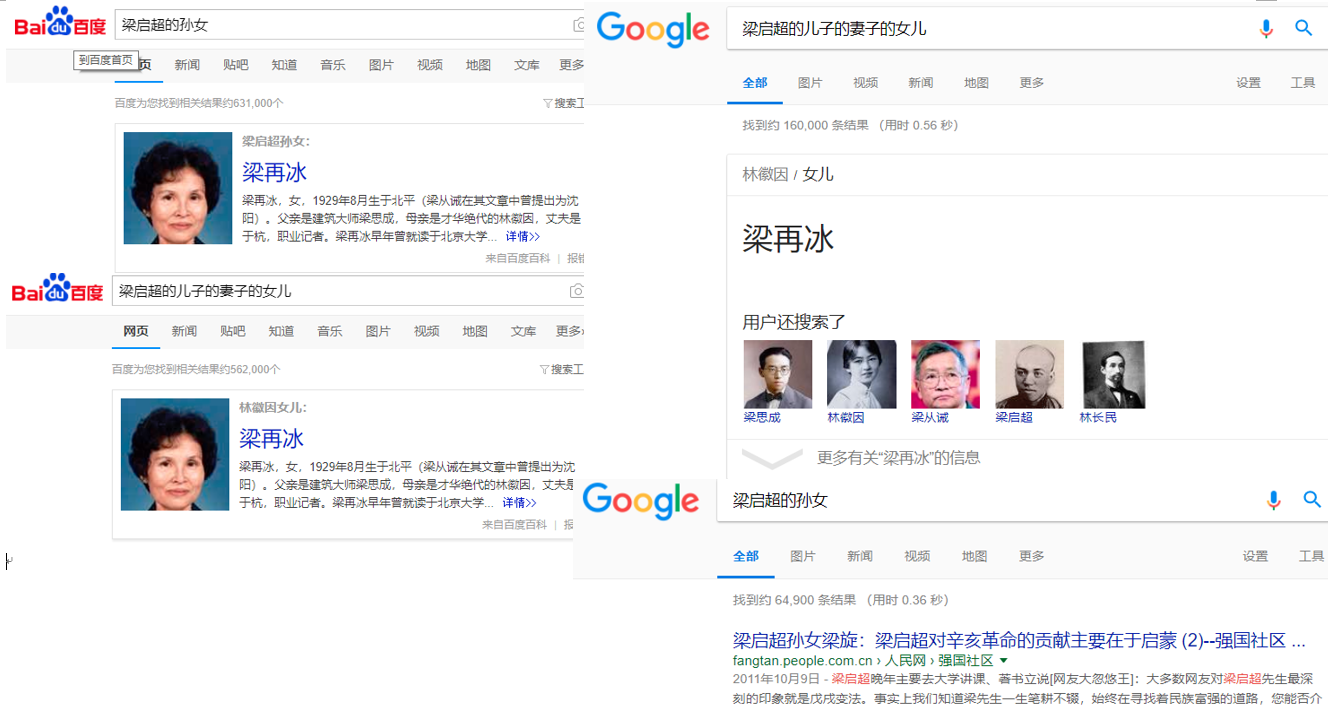
\includegraphics[width=\textwidth, bb= 0 0 1000 400]{pic/kg/kg_example1.png}
%		\caption{放置图片}
%		\label{0-001}
	\end{figure}
\end{frame}

\subsection*{如何生成知识图谱}
\begin{frame}
	\title {如何构建知识图谱}
	\begin{itemize}
		\item 手工构建
		\item 自动构建
		\begin{itemize} 
			\item 知识抽取:抽取实体和实体之间的关系
			\begin{itemize} 
				\item 实体抽取
				\item 关系抽取
				\item 属性抽取(珠穆朗玛峰)
			\end{itemize}
			\item 知识融合:整合相同义项,消歧义
			\item 知识加工:进行质量评估(可能有人工参与)将知识加入到知识库中
		\end{itemize}
	\end{itemize}

\end{frame}

\begin{frame}
	\begin{figure}[htbp]
		\centering
		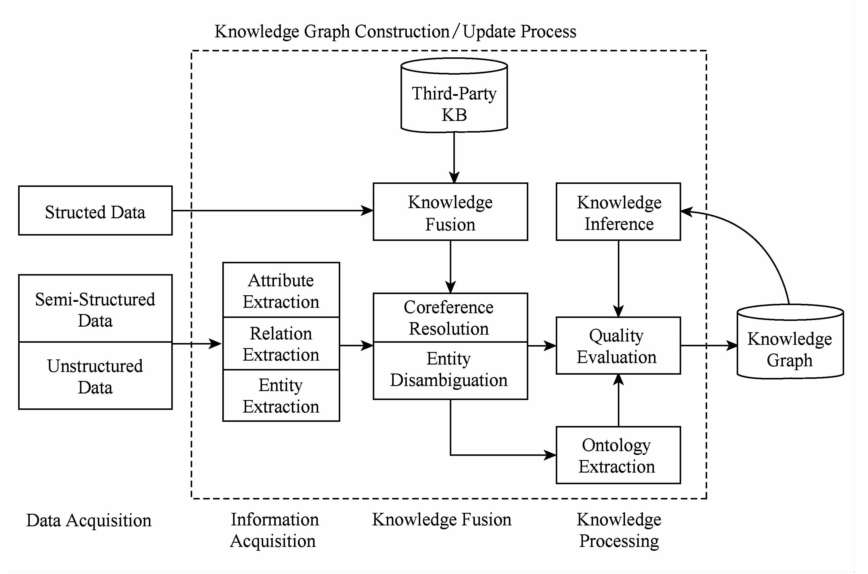
\includegraphics[width=\textwidth, bb= 0 0 600 400]{pic/kg/build_kg.png}
%		\caption{放置图片}
%		\label{0-001}
	\end{figure}
\end{frame}

\subsection*{自动生成错误的例子}
\begin{frame}
	\begin{figure}[htbp]
		\centering
		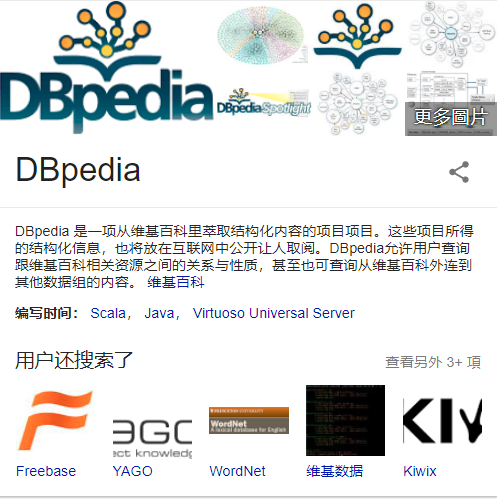
\includegraphics[width=0.5\textwidth, bb=0 0 400 400]{pic/kg/DBpedia_1.png}
		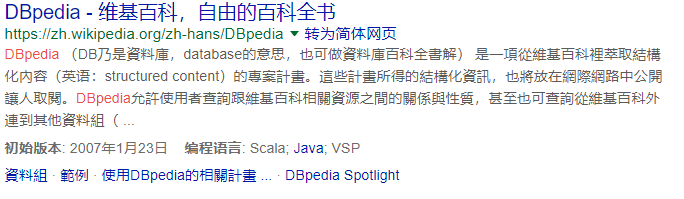
\includegraphics[width=0.5\textwidth, bb=0 0 400 400]{pic/kg/DBpedia_2.png}
	\end{figure}
	\begin{figure}[htbp]
		\centering
		
	\end{figure}
\end{frame}
\subsection*{Representation Learning}
\begin{frame}

	\begin{columns}
		\column{.5\textwidth}
			\begin{itemize}
				\item 之前所讲的是将Knowledge表示为图,但我们还可以表示为向量
				\item 实体是一个高维向量,关系也是一个高维向量			
			\end{itemize}
		\column{.5\textwidth}
			\begin{figure}[htbp]
				\centering
				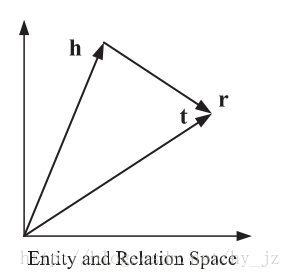
\includegraphics[width=1\textwidth, bb= 0 0 400 400]{pic/kg/transE.png}
			\end{figure}
	\end{columns}
	
\end{frame}

\begin{frame}
\begin{equation}
f_r(h,t) = -||\vec{h} + \vec{r} - \vec{t}||_{1/2}
\end{equation}
\end{frame}
